\documentclass[conference]{IEEEtran}

\usepackage{amsmath}
\usepackage{amssymb}
\usepackage{graphicx}
\usepackage{cite}

\title{Image Reconstruction in Inverse Problems: A Comparative Study of Tikhonov Regularization and Wiener Deconvolution}

\author{
	\IEEEauthorblockN{Mohammad Reza Shirkhan}
	\IEEEauthorblockA{
		M.Sc. in Electrical Engineering (Communication Systems)\\
		Email: r.shirkhan@gmail.com
	}
}

\begin{document}
	
	\maketitle
	
	\begin{abstract}
		Image reconstruction is a fundamental task in inverse problems, where the objective is to recover an unknown image from degraded observations. In this paper, a simple image reconstruction framework is studied using classical deconvolution methods. A clean grayscale image is degraded by Gaussian blur and additive Gaussian noise, and two reconstruction approaches are then applied: Tikhonov regularization and Wiener deconvolution. The performance of the methods is evaluated using Peak Signal-to-Noise Ratio (PSNR) and Structural Similarity Index (SSIM), together with visual inspection of the reconstructed images. Experimental results show that Wiener deconvolution slightly outperforms the selected baseline Tikhonov reconstruction in both PSNR and SSIM. In addition, a parameter sweep for the Tikhonov regularization coefficient reveals an important trade-off between numerical quality and perceptual sharpness.
	\end{abstract}
	
	\begin{IEEEkeywords}
		Inverse problems, image reconstruction, Tikhonov regularization, Wiener deconvolution, PSNR, SSIM, image deblurring
	\end{IEEEkeywords}
	
	\section{Introduction}
	Image degradation and restoration are central topics in signal processing, computer vision, and computational imaging. In many practical systems, the captured image is affected by optical blur, limited sensor resolution, motion, and random noise. As a result, the measured image differs from the original scene.
	
	Recovering the original image from a degraded observation is an inverse problem. Such problems are typically ill-posed, since the degradation process may remove information and amplify the effect of noise. Therefore, direct inversion is often unstable, and regularized reconstruction methods are required.
	
	Among classical reconstruction techniques, Tikhonov regularization and Wiener deconvolution are widely used because they are mathematically interpretable, computationally efficient, and suitable as baseline methods for more advanced reconstruction pipelines. In this work, both methods are implemented in Python and compared on a simple image deblurring task.
	
	\section{Problem Formulation}
	The image degradation process is modeled as
	\begin{equation}
		y = Hx + n
	\end{equation}
	where $x$ denotes the original image, $H$ is the blur operator, $n$ is additive noise, and $y$ is the observed degraded image.
	
	In the discrete setting, the blur operator is implemented as convolution with a point spread function. In this study, Gaussian blur is used to simulate the forward degradation process. After blurring, additive Gaussian noise is applied to obtain the final observation.
	
	The reconstruction problem consists of estimating $x$ from $y$. Since blur suppresses high-frequency image content and noise corrupts the observed signal, the inversion must be stabilized using appropriate reconstruction methods.
	
	\section{Reconstruction Methods}
	
	\subsection{Tikhonov Regularization}
	Tikhonov regularization reconstructs the unknown image by solving
	\begin{equation}
		\min_x \|Hx-y\|_2^2 + \lambda R(x)
	\end{equation}
	where $\lambda$ is the regularization parameter and $R(x)$ is a penalty term.
	
	In this work, derivative-based regularization is used:
	\begin{equation}
		R(x) = \|\nabla x\|_2^2
	\end{equation}
	which penalizes strong local variations in the reconstructed image. This improves numerical stability and suppresses noise amplification, but large values of $\lambda$ may oversmooth edges and fine image structures.
	
	The reconstruction is implemented in the Fourier domain for computational efficiency. A sweep over several values of $\lambda$ is performed to study the effect of regularization strength on reconstruction quality.
	
	\subsection{Wiener Deconvolution}
	Wiener deconvolution is a frequency-domain method that incorporates a noise-related stabilization term into the inversion:
	\begin{equation}
		X = \frac{H^*}{|H|^2 + K}Y
	\end{equation}
	where $Y$ is the Fourier transform of the observed image, $H$ is the Fourier transform of the blur kernel, $H^*$ denotes complex conjugation, and $K$ controls the balance between inversion and noise suppression.
	
	Compared with direct inversion, Wiener filtering is more robust in noisy conditions because it avoids excessive amplification of unreliable frequency components.
	
	\section{Experimental Setup}
	A sample image from the scikit-image dataset is used as the ground-truth image. The image is converted to grayscale and normalized to the range $[0,1]$. The degradation process consists of:
	\begin{enumerate}
		\item Gaussian blur with standard deviation $\sigma = 2$
		\item additive Gaussian noise with a fixed random seed for reproducibility
	\end{enumerate}
	
	The blurred and noisy image is reconstructed using both Tikhonov regularization and Wiener deconvolution. For the Tikhonov method, multiple values of $\lambda$ are tested:
	\begin{equation}
		\lambda \in \{0.01, 0.05, 0.1, 0.2, 0.5, 1, 2, 5, 10\}
	\end{equation}
	
	\section{Evaluation Metrics}
	
	\subsection{Peak Signal-to-Noise Ratio}
	PSNR is a standard full-reference metric derived from the mean squared error between the reconstructed image and the original image. Higher PSNR values indicate lower average pixel-wise reconstruction error.
	
	\subsection{Structural Similarity Index}
	SSIM measures similarity in terms of image structure, luminance, and contrast. Unlike PSNR, SSIM is more closely related to perceptual image quality. Values closer to 1 indicate better structural similarity.
	
	\section{Results}
	
	\subsection{Observed and Reconstructed Images}
	Fig.~\ref{fig:recon_a} shows the observed image together with the baseline Tikhonov reconstruction. Fig.~\ref{fig:recon_b} shows the Wiener reconstruction together with the best Tikhonov result selected from the parameter sweep.
	
	\begin{figure}[!t]
		\centering
		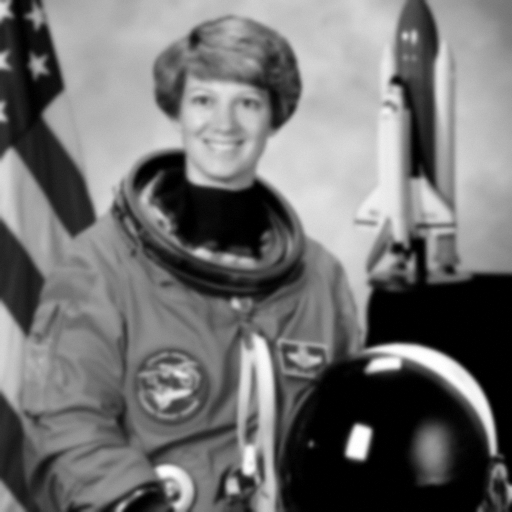
\includegraphics[width=0.45\linewidth]{results/observed.png}
		\hfill
		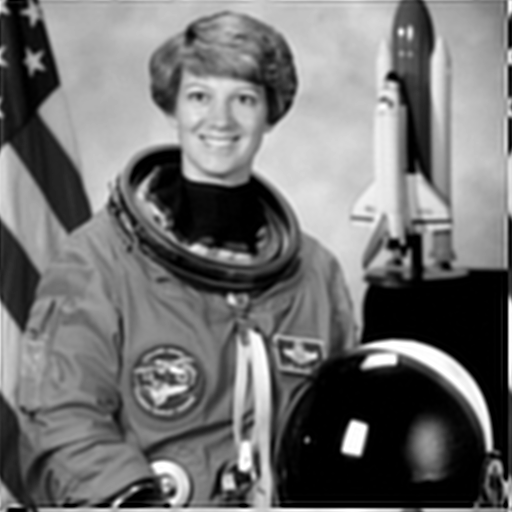
\includegraphics[width=0.45\linewidth]{results/tikhonov.png}
		\caption{Observed image (left) and baseline Tikhonov reconstruction (right).}
		\label{fig:recon_a}
	\end{figure}
	
	\begin{figure}[!t]
		\centering
		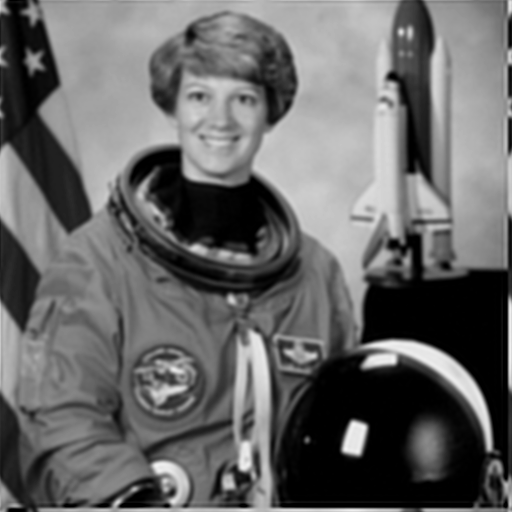
\includegraphics[width=0.45\linewidth]{results/wiener.png}
		\hfill
		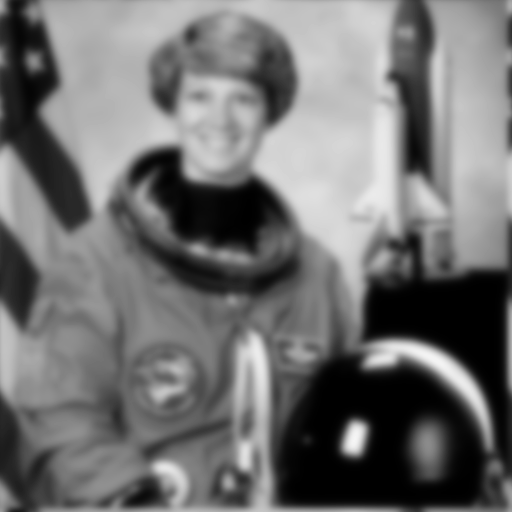
\includegraphics[width=0.45\linewidth]{results/best_tikhonov.png}
		\caption{Wiener reconstruction (left) and best Tikhonov reconstruction (right).}
		\label{fig:recon_b}
	\end{figure}
	
	\subsection{Quantitative Results}
	The baseline Tikhonov reconstruction produced a PSNR of 15.8998 and an SSIM of 0.4721. Wiener deconvolution achieved a PSNR of 15.9722 and an SSIM of 0.4861, indicating slightly better overall reconstruction performance in this experimental setup.
	
	\begin{table}[!t]
		\renewcommand{\arraystretch}{1.2}
		\caption{Quantitative comparison of reconstruction methods}
		\label{tab:mainresults}
		\centering
		\begin{tabular}{|c|c|c|}
			\hline
			Method & PSNR & SSIM \\
			\hline
			Tikhonov & 15.8998 & 0.4721 \\
			\hline
			Wiener & 15.9722 & 0.4861 \\
			\hline
		\end{tabular}
	\end{table}
	
	\subsection{Effect of the Tikhonov Regularization Parameter}
	To better understand the Tikhonov method, a parameter sweep over $\lambda$ was performed. The numerical results are listed in Table~\ref{tab:lambdasweep}, and the corresponding trends are shown in Fig.~\ref{fig:lambda_curves}.
	
	\begin{table}[!t]
		\renewcommand{\arraystretch}{1.2}
		\caption{Tikhonov parameter sweep}
		\label{tab:lambdasweep}
		\centering
		\begin{tabular}{|c|c|c|}
			\hline
			$\lambda$ & PSNR & SSIM \\
			\hline
			0.01 & 15.45 & 0.4304 \\
			\hline
			0.05 & 15.73 & 0.4603 \\
			\hline
			0.10 & 15.90 & 0.4721 \\
			\hline
			0.20 & 16.11 & 0.4849 \\
			\hline
			0.50 & 16.46 & 0.5039 \\
			\hline
			1.00 & 16.76 & 0.5183 \\
			\hline
			2.00 & 17.07 & 0.5296 \\
			\hline
			5.00 & 17.44 & 0.5343 \\
			\hline
			10.00 & 17.56 & 0.5219 \\
			\hline
		\end{tabular}
	\end{table}
	
	\begin{figure}[!t]
		\centering
		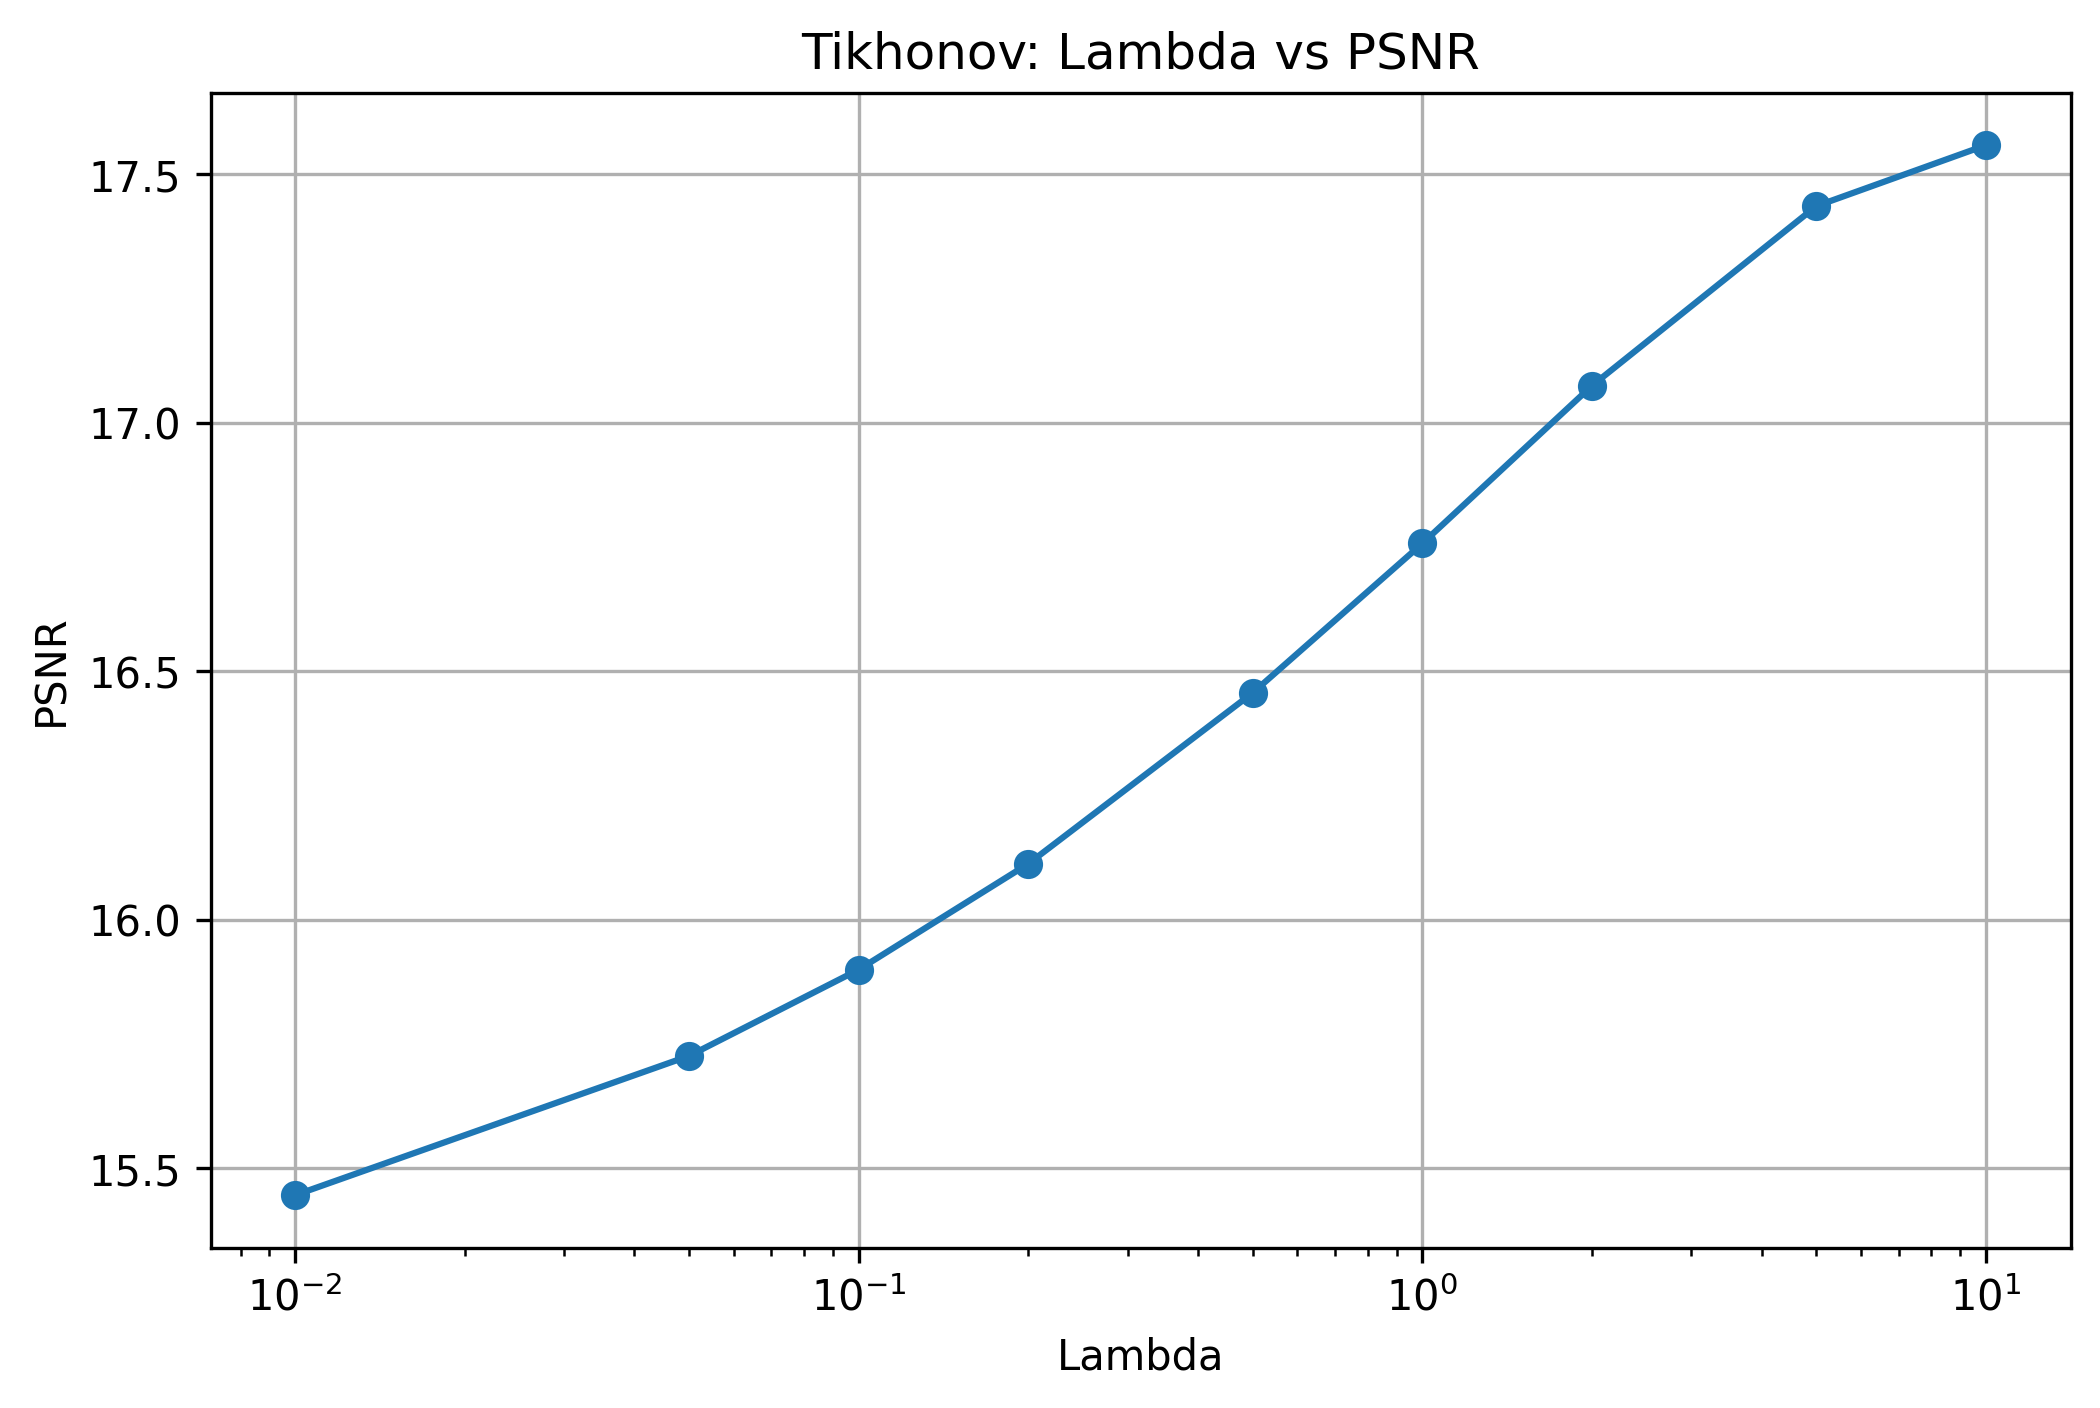
\includegraphics[width=0.45\linewidth]{results/lambda_psnr.png}
		\hfill
		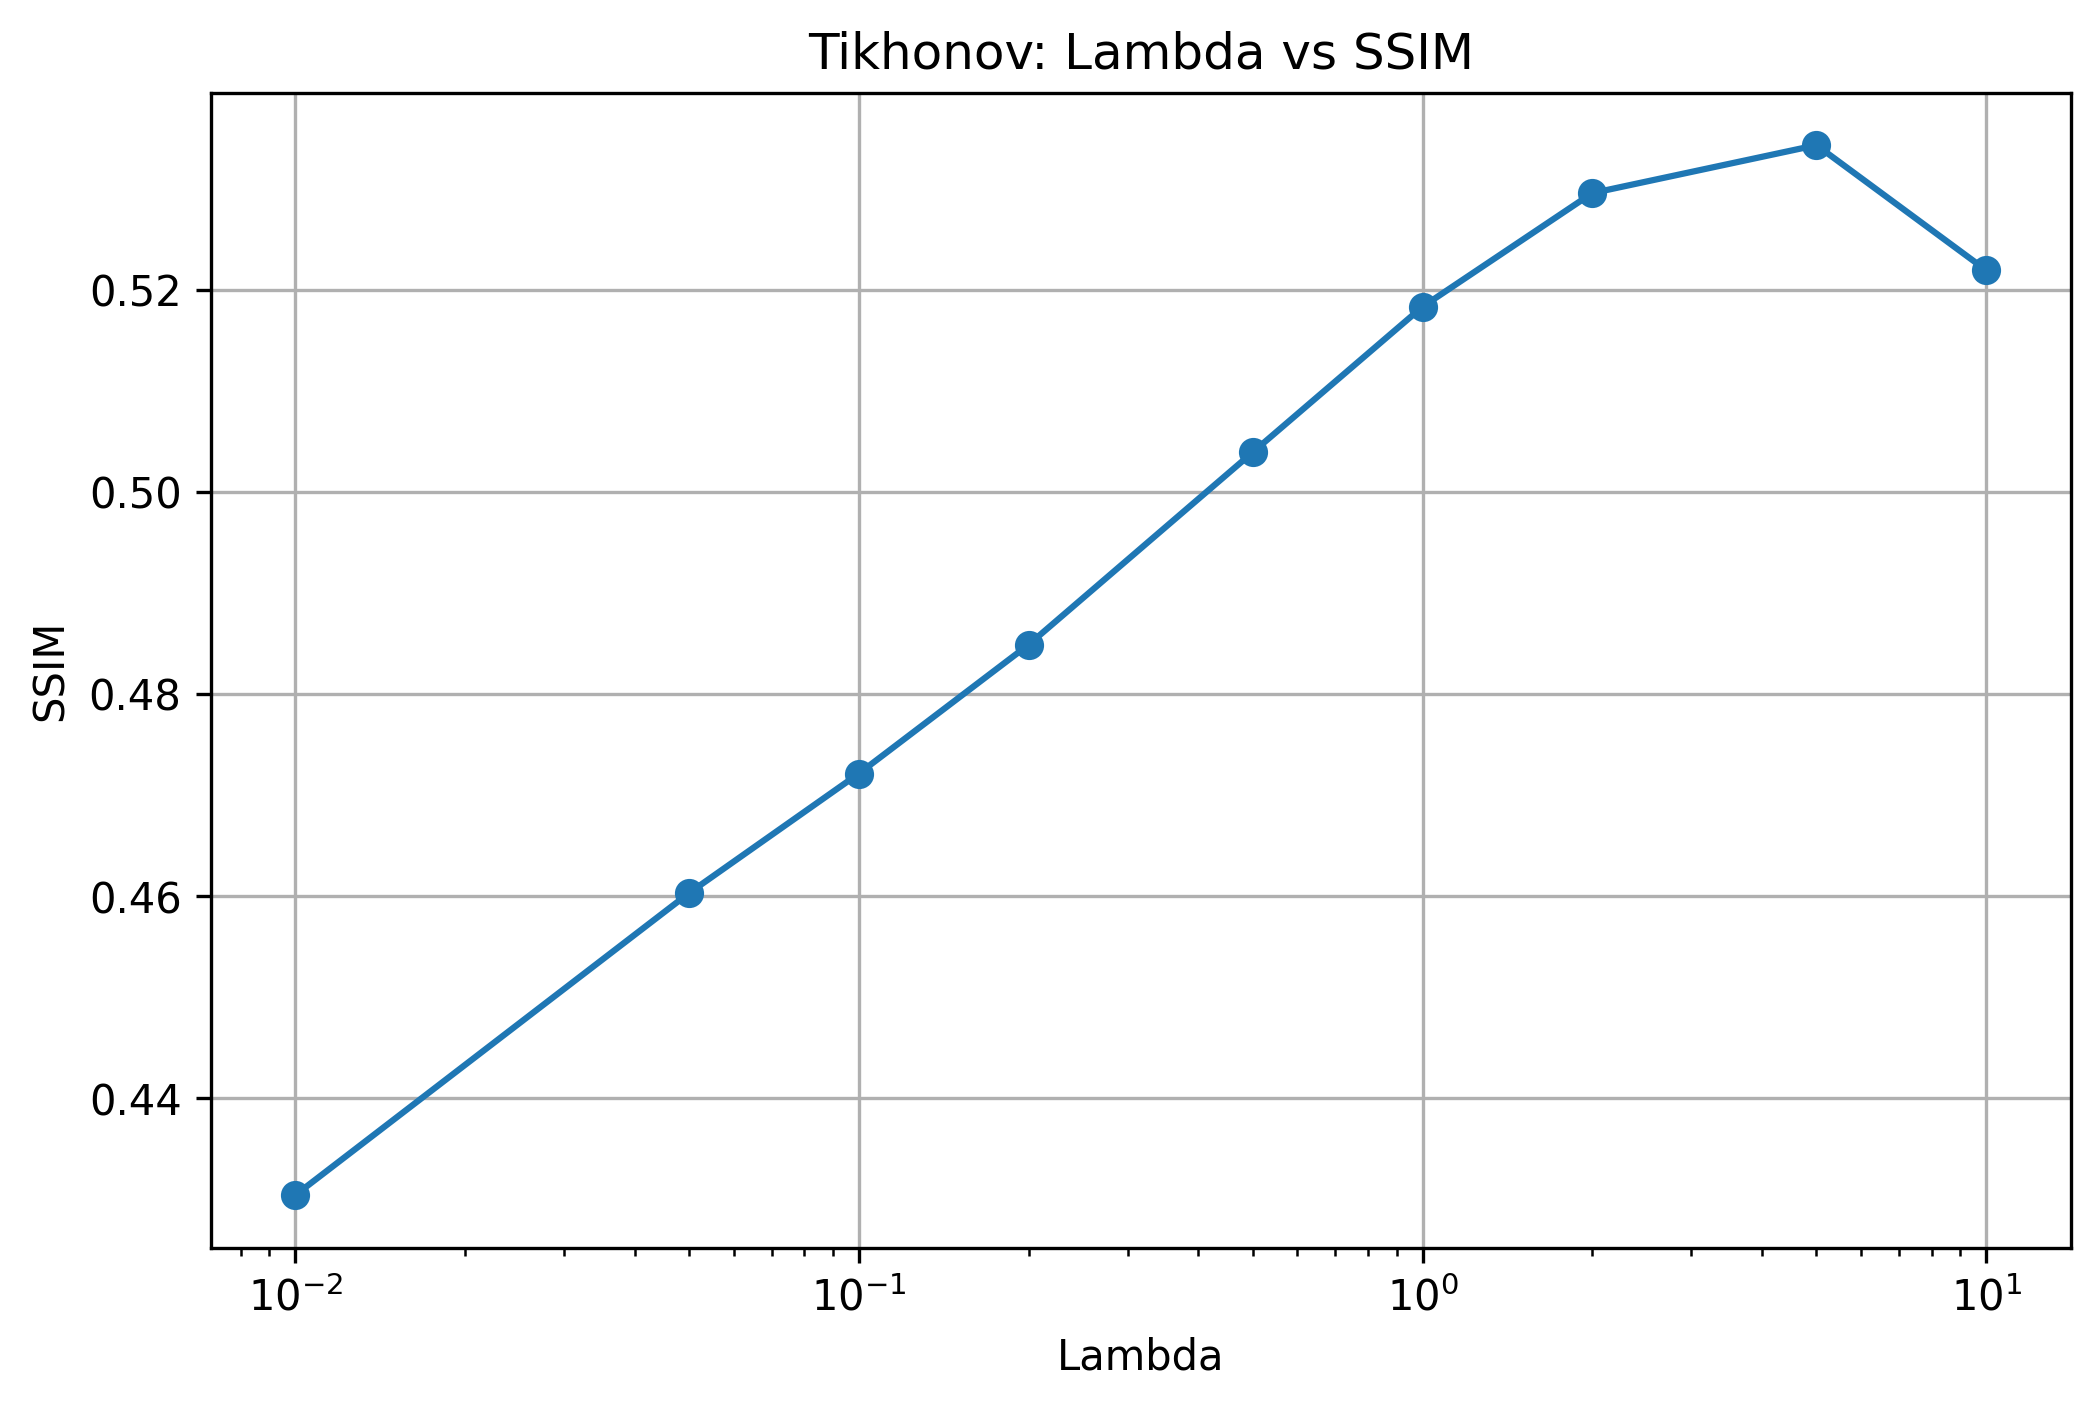
\includegraphics[width=0.45\linewidth]{results/lambda_ssim.png}
		\caption{PSNR (left) and SSIM (right) as functions of the Tikhonov regularization parameter $\lambda$.}
		\label{fig:lambda_curves}
	\end{figure}
	
	The highest PSNR was obtained at $\lambda = 10$, with a value of 17.56. However, the highest SSIM was obtained at $\lambda = 5$, with a value of 0.5343. This shows that the parameter that maximizes pixel-wise accuracy is not necessarily the same as the one that maximizes structural similarity.
	
	\section{Discussion}
	Several observations can be made from the experimental results.
	
	First, both reconstruction methods improve upon the blurred and noisy observation by partially inverting the degradation process. However, neither method fully restores high-frequency image details lost during blur.
	
	Second, the Tikhonov parameter sweep shows a clear regularization trade-off. As $\lambda$ increases, the reconstruction becomes more stable and both PSNR and SSIM initially improve. This indicates that stronger regularization effectively suppresses noise and stabilizes inversion. However, when $\lambda$ becomes too large, the reconstructed image becomes visually oversmoothed.
	
	Third, the experiments demonstrate that objective image quality metrics do not always agree with perceptual visual quality. Although $\lambda = 10$ produced the highest PSNR, visual inspection indicated that the corresponding image appeared overly smooth and less detailed. In contrast, intermediate values such as $\lambda = 5$ yielded a better balance between numerical performance and perceptual structure, as reflected by the higher SSIM. This experiment highlights a key limitation of PSNR as a reconstruction metric, as it may favor overly smooth solutions that lack perceptual sharpness.
	
	Finally, Wiener deconvolution slightly outperformed the baseline Tikhonov reconstruction in both PSNR and SSIM. This suggests that Wiener filtering can provide a more favorable balance between deblurring and noise suppression in this simple setup, although its performance remains limited by the severity of blur and the information loss inherent in the forward model.
	
	\section{Conclusion}
	This paper presented a simple image reconstruction study in the context of inverse problems using Gaussian blur and additive noise. Two classical reconstruction methods, Tikhonov regularization and Wiener deconvolution, were implemented and compared.
	
	The results showed that Wiener deconvolution slightly outperformed the baseline Tikhonov result in both PSNR and SSIM. A further sweep of the Tikhonov regularization parameter demonstrated that stronger regularization can improve numerical metrics, but excessive regularization produces oversmoothing and reduced visual sharpness.
	
	An important conclusion of this study is that reconstruction quality should not be judged using PSNR alone. Structural metrics such as SSIM, together with visual inspection, provide essential complementary information. Overall, this project serves as a useful baseline for understanding inverse problems and classical image reconstruction methods.
	
	\section*{Future Work}
	Future extensions of this work may include total variation regularization, blind deconvolution, non-Gaussian blur models, and learning-based reconstruction methods. Additional perceptual metrics could also be incorporated for a more comprehensive evaluation.
	
	\begin{thebibliography}{99}
		
		\bibitem{hansen}
		P. C. Hansen, J. G. Nagy, and D. P. O'Leary, \textit{Deblurring Images: Matrices, Spectra, and Filtering}. Philadelphia, PA, USA: SIAM, 2006.
		
		\bibitem{wiener}
		N. Wiener, \textit{Extrapolation, Interpolation, and Smoothing of Stationary Time Series}. Cambridge, MA, USA: MIT Press, 1949.
		
		\bibitem{gonzalez}
		R. C. Gonzalez and R. E. Woods, \textit{Digital Image Processing}, 4th ed. New York, NY, USA: Pearson, 2018.
		
		\bibitem{wang}
		Z. Wang, A. C. Bovik, H. R. Sheikh, and E. P. Simoncelli, ``Image quality assessment: From error visibility to structural similarity,'' \textit{IEEE Transactions on Image Processing}, vol. 13, no. 4, pp. 600--612, Apr. 2004.
		
	\end{thebibliography}
	
\end{document}